
\documentclass{jtetiproposalskripsi}

%-----------------------------------------------------------------
%Disini awal masukan untuk data proposal skripsi
%-----------------------------------------------------------------
\titleind{Sistem pemasaran Berbasis Web}
\fullname{AGUS ANDIKA FEBRIYANTO}

\idnum{1200631003}

\approvaldate{07 Februari 2015}

\degree{Sarjana Teknik Elektro}

\yearsubmit{2015}

\program{Manajemen Informatika}

\headprogram{Bagus Setya Rintyarna, S.T, M. Kom}

\firstsupervisor{Triawan Adi Cahyanto, M. Kom}
\firstnip{12 03 719}

\secondsupervisor{Bagus Setya Rintyarna, S.T, M. Kom}
\secondnip{09 03 521}


%-----------------------------------------------------------------
%Disini akhir masukan untuk data proposal skripsi
%-----------------------------------------------------------------

\begin{document}

\cover

\approvalpage

%-----------------------------------------------------------------
%Disini akhir masukan untuk muka skripsi
%-----------------------------------------------------------------

%-----------------------------------------------------------------
%Disini awal masukan Intisari
%-----------------------------------------------------------------
\begin{abstractind}
Dunia telah berubah dengan cepat seiring dengan perkembangan dan kemajuan di bidang teknologi, terutama teknologi informasi. Dengan hadirnya Internet yang telah berkembang pesat di seluruh dunia serta merubah cara hidup, berinteraksi, dan terutama berbisnis, khususnya dalam mengkomunikasikan strategi pemasaran perusahaan atau usaha. Dengan diperkenalkannya world wide web (www), Internet mampu menyediakan informasi tanpa batas ke seluruh dunia, sekalikgus memungkinkan terjadinya interaksi bisnis secara serentak tanpa adanya batas-batas negara, wilayah, serta waktu. Penggunaan internet secara komersil mewujudkan timbulnya pemasaran di internet serta perdagangan secara elektronik.
\paragraph{}
DI usaha yang saya jalani selama ini hususnya di bidang fotografi pemasarannya hanya dari mulut ke mulut saja dan di sekitar kecamatan dan sekitarnya saja. 
\paragraph{}
Dari permasalahan tersebut memunculkan gagasan untuk membuat suatu aplikasi berbasis web, yang di dalamnya dapat memberi informasi ke semua orang dan bagi yang berminat bisa langsung mendaftar di form yang telah di sediakan. Metodologi yang digunakan dalam pembuatan aplikasi ini adalah metode Waterfall. Bahasa pemrogramannya adalah PHP dan HTML. Untuk tampilan menggunakan CSS dan Jquery. Databasenya menggunakan MySQL. Tools dan Editor yang digunakan ialah XAMPP for Windows 7, Photoshop, Dreamweaver 8. 
\paragraph{}
Didukung dengan tersedianya jaringan internet lokal dan aplikasi ini nantinya akan digunakan sebagai media pemasaran.

\end{abstractind}
%-----------------------------------------------------------------
%Disini akhir masukan Intisari
%-----------------------------------------------------------------

\tableofcontents
\addcontentsline{toc}{chapter}{DAFTAR ISI}
\selectlanguage{bahasa}\clearpage\pagenumbering{arabic}\setcounter{page}{1}

%-----------------------------------------------------------------
%Disini awal masukan untuk Bab
%-----------------------------------------------------------------
\chapter{LATAR BELAKANG}

\section{Latar Belakang Masalah}
Perkembangan  teknologi, khususnya teknologi informasi komputer saat ini sudah semakin pesat. Informasi yang disajikan juga berdasarkan fakta dan dapat dipertanggungjawabkan. Seiring dengan  perkembangan tersebut membuat manusia menginginkan informasi tersebut didapat dengan cepat,  tepat, dan akurat. Maka dirancanglah sistem informasi yang terkomputerisasi, yaitu peralihan  dari  media penyampaian yang sifatnya manual menjadi lebih modern yang biasa kita sebut dengan teknologi internet. 
\paragraph{}
Dengan internet informasi dari seluruh lebih mudah didapatkan maupun disampaikan tanpa perlu datang ketempatnya langsung sehingga lebih efektif dan efisien. Selain itu pada saat ini teknologi tersebut didukung dengan media web sehingga  semakin memudahkan untuk saling berinteraksi bahkan melakukan transaksi bisnis. 
\paragraph{}
Website adalah sebuah sistem informasi yang ada pada server web yang memungkinkan penjelajah web untuk  mengakses informasi yang tersedia, dan web itu memiliki sifat statis dan dinamis. Web statis yaitu web yang  mempunyai ciri khas yang sangat  kentara. Isi dari web tersebut yaitu seperti teks,  gambar, tabel, link dan objek lainnya. Sedangkan web dinamis yaitu web yang mampu menyesuaikan dari tahap faktor tertentu dan mampu memberikan apa yang diminta oleh pengunjung.
\paragraph{}
Dengan adanya website yang dapat diakses secara luas, dimanapun dan kapanpun online selama 24 jam. Hal inilah yang menyebabkan banyak lembaga pendidikan, instansi negeri, swasta, personal profil organisasi baik bisnis maupun non bisnis untuk memperkenalkan dan mempromosikan tujuan keberadaan mereka.
\paragraph{}
Studio foto Jember Photoshop perlu dibuat sebuah website guna meningkatkan kualitas dan kemajuan perusahaan. Berdasarkan survey yang telah penulis lakukan pada Studio foto Jember Photoshop,  ternyata  masih  banyak kendala  serta  kekurangan dalam memasarkan jasa dan karya hasil foto. Solusi dari permasalahan tersebut adalah suatu layanan yang mampu menyediakan semua informasi tentang jasa-jasa yang tersedia  pada Studio foto Jember Photoshop yang dapat diperoleh dengan mudah, cepat dan akurat. Dengan alasan inilah kami membangun layanan informasi dan jasa berbasis web dengan mengambil  judul “Sistem Informasi Pemasaran Berbasis Web Sebagai Media Promosi”.



\section{Rumusan Masalah}
Dengan memperhatikan latar belakang yang telah disampaikan sebelumnya, maka rumusan masalahnya adalah sebagai berikut : 
\begin{itemize}
\item[-]Konsumen yang mengalami kesulitan memperoleh  informasi  mengenai hasil foto untuk menjadikan contoh konsep pemptretan.
\item[-]Kurang efisien dari segi pemesanan karena menunggu konsumen datang di studio foto terlebih dahulu.
\end{itemize}

\section{Identifikasi Masalah}
Bagaimana  cara  membangun  sebuah  aplikasi  berbasis web sebagai  media promosi atau pemasaran yang dapat memberikan serta menyajikan informasi yang efektif serta jasa yang menarik dan bermanfaat untuk Studio Foto Jember Photoshop ?

\section{Tujuan}
Berdasarkan latar belakang, mengidentifikasikan perumusan masalah sebagai berikut :
\begin{itemize}
\item[-]Memudahkan fotografer mempromosikan hasil pemotretan ke konsumen.
\item[-]Memberikan informasi – informasi perkembangan terbaru studio dan memberikan pengetahuan di bidang fotografi.
\end{itemize}

\section{Manfaat}
\begin{itemize}
\item[1.]Mempemudah konsumen untuk mengetahui hasil pemotretan. 
\item[2.]Mempermudah konsumen untuk mengetahui info terbaru dari studio foto Jember Photoshop.

\end{itemize}


%-------------------------------------------------------------------------------
\chapter{LANDASAN TEORI}                

\section{Teori Tentang Permasalahan}
Menjelaskan secara teoritis tentang permasalahan untuk mendukung perangkat lunak pemasaran berbasis web.
\subsection{Aplikasi}
Definisi aplikasi menurut Jack Febrian (2007:35) :
''\textit{Program aplikasi atau program siap pakai. Program yang direka untuk melaksanakan suatu fungsi bagi pengguna atau aplikasi yang lain. Contoh-contoh aplikasi ialah program pemproses kata dan Web Browser.} '' 
\paragraph{}
Dari definisi diatas dapat diartikan bahwa aplikasi merupakan program yang siap pakai atau juga siap digunakan dan juga program yang dimaksud memiliki proses tertentu  sebagaimana pengguna membutuhkannya misalnya proses dari kata ataupun yang lainnya.


\subsection{Web}
Pengertian  web  menurut  Sudarso  (2008)  :
''\textit{Website atau situs dapat diartikan sebagai kumpulan halaman halaman yang digunakan untuk menampilkan informasi teks, gambar diam atau gerak, animasi, suara, dan atau gabungan dari semuanya itu baik yang bersifat statis maupun dinamis yang membentuk satu rangkaian bangunan yang saling terkait dimana masing-masing dihubungkan dengan jaringan-jaringan halaman ( hyperlink )}.''
\paragraph{}
Dari pengertian Website diatas dapat diartikan bahwa website sebagai kumpulan dari halaman-halaman situs, yang terangkum dalam sebuah domain  ataupun subdomain,  yang  tempatnya  berada  di  dalam  World  Wide  Web  (  WWW  )  di internet.

\section{Bahasa Pemrograman Web}
\subsection{PHP }
Menurut Prasetio Adi (2012), Menyebutkan Bahwa : \textit{''PHP  (PHP:  Hypertext  Preprocessor)  adalah  bahasa  script yang ditanam disisi server. kalau kita pake istilah sehari-hari,munkin seperti ini: prosesor PHP dijalankan di server (Windows atau Linux). Saat sebuah  halaman  dibuka  dan mengandung  kode  PHP,  prosesor  itu  akan menerjemahkan  dan mengeksekusi  semua  perintah  dalam  halaman  tersebut,  dan kemudian  menampilkan  hasilnya  ke  browser  sebagai halaman HTML biasa.''}
\paragraph{}
PHP  (Personal  Home  Page)  adalah  script  yang  paling  banyak  dipakai  saat  ini. PHP banyak dipakai untuk meprogram situs web dinamis, walaupun tidak tertutup kemungkinan digunakan untuk pemakaian lain. Kelebihan PHP dari bahasa Pemrograman lain adalah :
\begin{itemize}
\item[1]HP  adalah  sebuah  script  yang  tidak  melakukan  sebuah  kompilasi  dalam penggunaannya. 
\item[2]Web Server yang mendukung PHP dapat ditemukan dimana-mana dari mulai Apache,  IIS,  Lighttpd,  hingga  Xitami  dengan  konfigurasi  yang  relative mudah
\item[3]Dalam  sisi  pengembangan  lebih  mudah,  karena  banyaknya  milis-milis  dan developer yang siap membantu dalam pengembangan. 
\item[4]Dalam  sisi  pemahaman,  PHP  adalah  bahasa  scripting  yang  paling  mudah karena memiliki referensi yang banyak
\item[5]PHP  adalah  bahasa  open  source  yang  dapat  digunakan  di  berbagai  mesin (Linux,  Unix,  Macintosh,  Window)  dan  dapat  dijalankan  secara runtime melalui console serta juga dapat menjalankan perintah-perintah sistem.
\item[6]PHP: Hypertext Preprocessor adalah bahasa skrip yang dapat ditanamkan atau disisipkan  ke  dalam HTML.  PHP  banyak  dipakai  untuk  memrogram situs web dinamis. PHP dapat digunakan untuk membangun sebuah CMS.
\end{itemize}

\subsection{HTML}
Menurut Handayani Mierna Puspa, menyebutkan bahwa : 
\textit{''Hypertext Markup Language (HTML) adalah bahasa yang digunakan untuk menulis halaman  web. HTML merupakan pengembangan  dari  standar pemformatan dokumen  teks  yaitu Standard Generalized Markup Language (SGML). HTML sebenarnya adalah dokumen ASCII atau teks biasa,  yang dirancang untuk tidak tergantung pada satu system operasi tertentu.''}

\paragraph{}
Hypertext  Markup Language (HTML) adalah  bahasa  yang  digunakan untuk menulis halaman web. HTML merupakan pengembangan dari standar pemformatan  dokumen teks yaitu Standard Generalized Markup  Language (SGML).  HTML  sebenarnya adalah dokumen  ASCII  atau  teks  biasa,  yang dirancang untuk tidak tergantung pada suatu sistem operasi tertentu. Mendesain  HTML  berarti  melakukan  suatu  tindakan  pemrograman. Namun HTML  bukanlah  sebuah  bahasa  pemrograman.  Namun  HTML hanyalah  berisi perintah-perintah yang telah terstruktur berupa tag-tag penyusun. Menuliskan tagtag  HTML  tidaklah  sebatas  hanya  memasukkan perintah-perintah  tertentu  agar HTML kita dapat di akses oleh browser. Mendesain HTML adalah adalah sebuah seni  tersendiri.  Homepage  yang merupakan  implementasi  dari  HTML  adalah refleksi dari orang yang membuatnya. Untuk itu kita perlu mendesainnya dengan baik agar para pengunjung  homepage  yang  kita  buat  merasa  senang  dan bermanfaat. 
Mendesain  HTML  dapat  dilakukan  dengan  dua  cara: 
\begin{itemize}
\item[1]Menggunakan  HTML  Editor,  seperti  Microsoft  FrontPage,  Adobe Dreamweaver,  dan  lain-lain.  Dapatkan  editor  HTML  lainnya  disini. 
\item[2]Dengan cara menuliskan sendiri secara manual satu persatu tag-tag HTML ke dalam dokumen HTML
\end{itemize}

\section{Database yang digunakan}
\subsection{MySQL}
Pengertian  MySql  menurut  (Kadir,  2009,  p.  15):
''MySql  merupakan software yang tergolong  database  server  dan bersifat Open  Source.  Open  Source menyatakan bahwa  software  ini dilengkapi  dengan  source  code  (kode  yang dipakai  untuk  membuat MySql).''

\paragraph{}
MySQL adalah suatu sistem manajemen basis data relasional (RDBMS-Relational Database System) yang mampu bekerja dengan cepat, kokoh, dan mudah digunakan. Contohlah RDBMS lainnya adalah Oracle,  Sybase.  Basis Data memungkinkan kita untuk menyimpan, menelusuri, mengurutkan dan mengambil data secara efisien. Server MySql yang akan membantu melakukan fungsionalitas tersebut. 

\section{Alat Bantu Sistem }
\subsection{XAMPP}
Pengertian XAMPP menurut (Nugroho, Pengenalan XAMPP 2008) : 
''XAMPP merupakan paket PHP yang berbasis Open Source yang dikembangkan oleh sebuah komunitas Open Source. Dengan menggunakan XAMPP anda tidak usah bingung untuk melakukan penginstallan program-program yang lain, karena semua kebutuhan telah disediakan oleh XAMPP.''

\paragraph{}
XAMPP atau X (Cross Platform)  Apache MySQL PHP Perl adalah sebuah perangkat lunak (software) yang dibuat oleh tim dari Apache Friends (www.apachefriends.org) yang fungsinya adalah untuk menjalankan  program PHP, MySQL dan Perl dalam satu waktu yang bersamaan. XAMPP memudahkan para web developer untuk mengembangkan dan membuat sebuah website di local PC/Laptop, sehingga proses pembuatan sebuah website menjadi lebih aman dan cepat dibandingkan melakukan proses pembuatan website lewat online server.


\chapter{ANALISIS DAN PERANCANGAN PERANGKAT LUNAK}
\section{Gambaran Umum Perusahaan}
Jember photoshop merupakan perusahaan yang berdiri dibidang jasa maupun penjualan dalam bentuk kewirausahaan. Pemilik dari Salsha Photo Studio  Asep Wawan selalu mencoba dan berusaha untuk melayani konsumen secara profesional dan kepuasan pelanggan. Jember photoshop Studio ini berdiri pada April 2011. Awal mula berdiri, pemilik dari Jember photoshop memiliki  hobi  dalam  editing  foto dan fotografi sehingga  tercipta  ide  untuk  membuat  usaha  cetak, editing foto dan jasa fotografer.
\subsection{Struktur Organisasi Perusahaan}


\begin{table}[ht!]
  \centering
    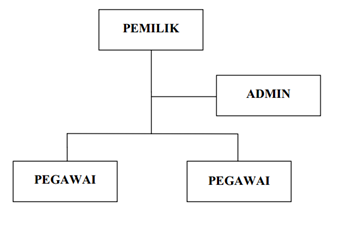
\includegraphics[width=0.6\textwidth]{gambar/struktur}
    \caption{Struktur Organisasi Perusahaan Salsha Photo Studio}
    \label{wsn}
\end{table}
\newpage

\paragraph{}
Kegiatan di Jember photoshop Studio ini dalam sehari-hari hingga sekarang melayani pelanggan dalam kebutuhan percetakan, pengeditan, foto dan pemotretan, yang berlokasi di Jl. A.yani no.75 D Wuluhan. 


\subsection{Visi dan Misi Perusahaan}
\begin{itemize}
\item[] Visi  :  Menjadi  bahan  usaha  yang  terdepan  dalam  usaha  percetakan  (print) foto atau  data  yang  menjungjung  tinggi  profesionalisme  dalam  berkarya  dan memuaskan konsumen.
\item[]Misi  :  Menerapkan  aplikasi  teknologi  software maupun hardware yang  anggih dan  modern  dalam  dunia  cetak  atau  editing  foto  serta  editing  data  dengan tetap berpijak pada kecepatan pelayanan untuk kepuasan konsumen.
\end{itemize}


\section{Analisis Fungsional }
Penulis membuat perangkat lunak web  yang untuk mempromosikan produk dan jasa melalui web JEMBER PHOTOSHOP STUDIO. Periklanan untuk promosi ini jarang dilakukan dan pemilik perusahaan beserta penulis memanfaatkan hal tersebut untuk mengembangkan periklanan untuk mengiklankan perusahaan dengan menggunakan web, dimana penulis menggunakan bahasa pemrograman PHP, dengan menggunakan Phpmyadmin yang ada di program xampp. Gambaran umum yang terdapat pada perangkat lunak web ini yaitu : 
\begin{itemize}
\item[1]Header,  memberikan  informasi  tema  dengan  nama  perusahaan  yang ditampilkan.

\item[2]Skema navigasi, navigasi  yang digunakan ialah  navigasi  yang diterapkan di bagian atas dan di bagian kiri, navigasi bagian atas menghubungkan kepada halaman-halaman utama website seperti home yang  menyambungkan sedangkan  navigasi  bagian  kiri  menghubungkan  ke  informasi  atau halaman yang lebih rinci. Halaman-halaman pada navigasi bagian atas : 
\begin{itemize}
\item[a]Home, menampilkan halaman utama dari web informasi produk terbaru
\item[b]Profil, menampilkan menampilkan profil tentang perusahaan.
\item[c]Cara Pembelian, memberikan informasi tentang tata cara pembelian.
\item[d]Produk, menampilkan barang-barang yang akan diperjualkan. Sedangkan untuk  navigasi  bagian  kiri  menampilakan  halaman-halaman katagori dari produk, produk best seller, dan banner iklan . 
\end{itemize}
\item[3]Main Body atau bagian isi web, isi dari informasi-informasi pada setiap halaman.
\item[4]Footer atau bagian bawah web, mencantumkan nama perusahaan.
\end{itemize}



\begin{thebibliography}{9}

\bibitem[satu(2015)]{satu01}
Jogiyanto, H.M, 2001. \textit{Analisis dan Desain Sistem Informasi}. Yogyakarta : Penerbit Andi Offset. 

\bibitem[dua(2015)]{dua02}
Kristanto Andri. 2007. \textit{Perancangan Sistemdan Aplkasinya}. Yogyakarta : Penerbit Gava
Media. 

\bibitem[tiga(2015)]{tiga03}
Mc, Leod Raymon. 2008. \textit{Management Information System. Edisi 10}. Pearson/Prentice Hall.  Bacon. J., "Practical PHP and MySQLBuilding 


\bibitem[empat(2015)]{empat04}
Eight Dynamic Web Applications", November 2006. Coggeshall, J., PHP 5 Unleashed, Sams, 28 December 2004.


\bibitem[enam(2015)]{enam06}
Hayder. H.,  “Object-oriented Programming with PHP5", Desember 2007 

\bibitem[tujuh(2015)]{tujuh07}
 Nugroho, B., Aplikasi Pemrograman Web Dinamis dengan PHP dan MySQL, Cetakan
Pertama, 2004. 

\bibitem[delapan(2015)]{tujuh08}
 Lerdorf. R., P. Maclntyre. , and K. Tatroe. “Programming PHP, 2

\end{thebibliography}
\addcontentsline{toc}{chapter}{DAFTAR PUSTAKA}
%-----------------------------------------------------------------
%Disini akhir masukan Daftar Pustaka
%-----------------------------------------------------------------

\end{document}